
%%%%%%%%%%%%%%%%%%%%%%%%%%%%%%%%%%%%%%%%%%%%%%%%%%%%%%%%%%%
% --------------------------------------------------------
% Tau
% LaTeX Template
% Version 2.4.3 (01/09/2024)
%
% Author: 
% Guillermo Jimenez (memo.notess1@gmail.com)
% 
% License:
% Creative Commons CC BY 4.0
% --------------------------------------------------------
%%%%%%%%%%%%%%%%%%%%%%%%%%%%%%%%%%%%%%%%%%%%%%%%%%%%%%%%%%%

\documentclass[9pt,a4paper,twoside]{tau-class/tau}
\usepackage[english]{babel}

%----------------------------------------------------------
% TITLE
%----------------------------------------------------------

\journalname{Aprenentatge Computacional}
%% TODO: Optional, you can set a fancier title if you like
\title{Sign Language ASL Recognition using Bag of Visual Words and Super Vector Machines}

%----------------------------------------------------------
% AUTHORS, AFFILIATIONS AND PROFESSOR
%----------------------------------------------------------

%% TODO: Set your names here
\author[a]{Samuel Ortega Cuadra}
\author[b]{Laia Alexandra Sjöberg Cerezo}

%----------------------------------------------------------

\affil[a]{1669776}
\affil[b]{1667894}


%----------------------------------------------------------
% FOOTER INFORMATION
%----------------------------------------------------------

\institution{Universitat Autònoma de Barcelona}
\footinfo{Class Project}
\theday{December 10, 2024}
\leadauthor{Group XX} 		%% TODO: Set your group ID here
\course{Aprenentatge Computacional}

%----------------------------------------------------------
% ABSTRACT AND KEYWORDS
%----------------------------------------------------------

\begin{abstract}    
	%% TODO: Change this default abstract into something nice that describes your work.
	%% Keep it below 300 words.
    This project focuses on developing a system for recognizing American Sign Language (ASL) alphabet and numbers. The proposed approach combines image preprocessing, feature extraction, and prediction models to accurately classify hand gestures. The dataset consists of images of hands representing ASL letters and numbers, which are processed by isolating the hand region, converting it in grayscale and applying a mask for feature extraction. Dense SIFT and a Bag of Words model are used to create feature representations, and a Support Vector Machine (SVM) classifier is trained and optimized through grid search for maximum accuracy.
    
    The finished system can recognize hands by retrieving frames from video input, and translating ASL gesture sequences into coherent text. 
    
    This work lays a foundation for future developments in sign language recognition and improving accessibility for the deaf community by providing a tool for real-time translation of sign language to text.
\end{abstract}

%----------------------------------------------------------

%% TODO: Set appropriate keywords for your report.
\keywords{a, b, c, d}

%----------------------------------------------------------

\begin{document}
	%% Do NOT change any of this. Line numbers should be kept.
    \maketitle 
    \thispagestyle{firststyle} \tauabstract 
    \tableofcontents
    \linenumbers 
    
%----------------------------------------------------------

\section{Introduction}

    \taustart{T}his document presents the development of a system for recognizing American Sign Language (ASL) alphabet and numbers. It outlines the steps taken to achieve this goal, from the \textbf{dataset collection} and preprocessing to the implementation of a \textbf{Bag of Visual Words} to help builiding a \textbf{SVM model} for classification. The system is then extended to \textbf{process videos}, extract frames, identify ASL symbols, and \textbf{reconstruct} the words being spelled.
\section{Finding The Dataset}

	When looking for a good ASL dataset, we found the \href{https://www.kaggle.com/datasets/ayuraj/asl-dataset}{American Sign Language Dataset} dataset on Kaggle. This dataset contains 2515 images of 400x400 pixels, each showing a hand making an ASL letter or number. The dataset is divided into 36 folders, one for each letter of the alphabet and one for each of the numbers from 0 to 9. The images are in JPEG format and have a black background with a white hand. The dataset is well-organized and easy to use, making it a good choice for our project.

    \subsection{Dataset Preprocessing}

    The preprocessing of the dataset invloves the following steps: 
    \begin{enumerate}
        \item \textbf{Dataset Organization}: The dataset is organized into folders, one for each letter of the alphabet and one for each number from 0 to 9. Each folder contains 65 to 70 images of hands making the corresponding ASL symbol. A \textit{categories} dictionary was created to map each label to its corresponding folder name. The filenames of all images were collected and combined with their respective category labels to construct a DataFrame.
        \item \textbf{Shuffiling the Dataset}: To avoid any bias in the training and testing data, the dataset was shuffled. This ensures that the data is randomly distributed and that the model will not be trained on any specific order of images.
        \item \textbf{Image Loading}: Each image was loaded from its respective path and converted into a NumPy array. Providing a new variable with a structured representation of pixels called \textit{pixel\_ data}.
        \item \textbf{Grayscale conversion}: The images were converted to grayscale to reduce the complexity of the model and improve training speed.
    \end{enumerate}


    \subsection{Masking the Hand}
    In order to find the best features we tried to mask the hand in the image using differents methods. The optimal resulting
    method was surprisingly the easiest. We took a look at the first 20 pixels of the image before converting it to grayscale and we found the most frequent color. Sequently, we applied a
    standard deviance and removed all of the background with the same colours, which will be really important when extracting the keypoints in the next chapter.
    \begin{info}
        We tried other methods such as brightness threshold, gaussian blur and several others from the computer vision library. They all ended up 
        being less efficient than the one we finally used.
    \end{info}
		
\section{Feature extraction} \label{sec:table}

    \subsection{Figures}
		
	Fig. \ref{fig:figure} shows an example figure. Figures can be referenced using \verb|\ref{ident}|, where \texttt{name} is a previously-defined \verb|\label{name}| for any object in the document. You can actually also do this with sections (Section \ref{sec:table}) or equations or other types of objects that will be seen below.
		
	\begin{figure}[H]
		\centering
		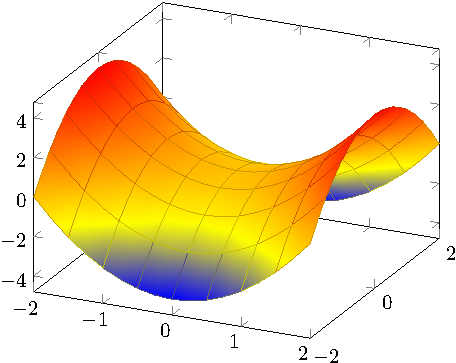
\includegraphics[width=0.75\columnwidth]{Example.pdf}
		\caption{Example figure obtained from PGFPlots \cite{PFGPlots}.}
		\label{fig:figure}
	\end{figure}
		
        Fig. \ref{fig:examplefloat} shows an example of two figures that cover the width of the page. It can be placed at the top or bottom of the page. The space between the figures can also be changed using the \verb|\hspace{Xpt}| command.
		
        \begin{figure*}[tp] % t for position at the top of the current page; b for position at the bottom; p for new page
		\centering
		  \begin{subfigure}[b]{0.38\linewidth} % Fig (a)
			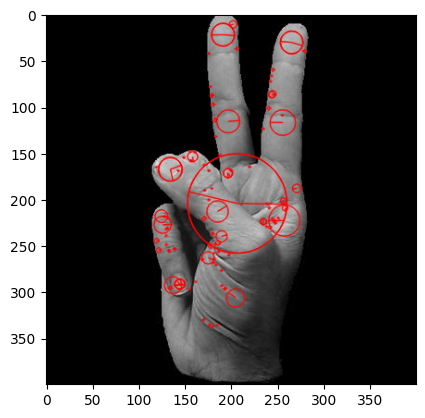
\includegraphics[width=\linewidth]{firstfeatureextraction.png}
			\caption{Example left figure.}
			\label{fig:figa}
		\end{subfigure}
			\hspace{20pt}   % Space between the figures
		\begin{subfigure}[b]{0.375\linewidth} % Fig (b)
			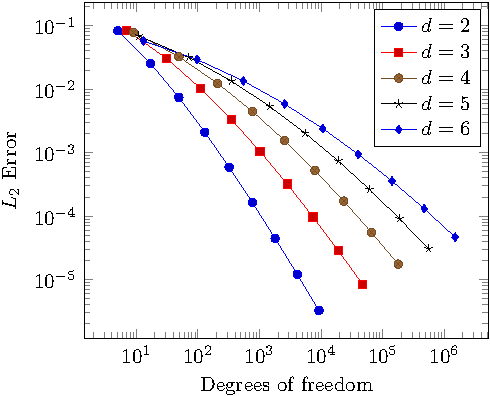
\includegraphics[width=\linewidth]{Example3.pdf}
			\caption{Example right figure.}
			\label{fig:figb}
		\end{subfigure}
		\caption{Example figure that covers the width of the page obtained from PGFPlots \cite{PFGPlots}.}
		\label{fig:examplefloat}
	\end{figure*}

    \begin{info}
    	Figures in \LaTeX are known to be quite anarchic. You should always wait until the very end to place them well into the document. In any case, you should always reference the Figure and provide a Caption so that it can be contextualised even when it lies far away from the text that accompanies it.
    \end{info}

    \begin{info}
    	Avoid raster graphics (jpeg, png) for figures if you can. Always use vectorial formats for plots and diagrams. The preferred formats for vectorial images are SVGs converted to Encapsulated Post-Script (.eps, you can use Inkscape to perform this conversion) or PDF files. Regardless of the image format you are using, generate reasonably high-resolution files (the usual is 300dpi, which means 300 pixels per squared inch). \textbf{Keep in mind that Matplotlib can be configured to generate plots with these settings.}
    \end{info}

    \subsection{Tables}
	
        Table \ref{tab:table} shows an example table. The \verb|\tabletext{}| is used to add notes to tables easily. 

        \begin{info}
        	This template uses the \texttt{booktabs} package by default. This package makes typesetting nice tables easier, but it imposes some general design guidelines. The most prominent is the distinction between middle and edge rules (horizontal lines) and the discouragement of vertical lines.
        \end{info}

        \begin{info}
        	You should \textbf{always} avoid typesetting tables by hand. Use tools such as \href{https://www.tablesgenerator.com/}{this one} to spare yourself some unnecessary pain.
        \end{info}
		
	\begin{table}[H]
		\centering
		\caption{Small example table.}
		\label{tab:table}
		\begin{tabular}{cc}
			\toprule
			\textbf{Column 1} & \textbf{Column 2} \\
			\midrule
			Data 1 & Data 2 \\
			Data 3 & Data 4 \\
			\bottomrule
		\end{tabular}
			
            \tabletext{Note: I'm a table text for additional information.}
			
	\end{table}
		
\section{Predicting using the codebook}

    \subsection{Tauenvs}
	
        This template has its own environment package \textit{tauenvs.sty} designed to enhance the presentation of the document. Among these custom environments are \textit{tauenv}, \textit{info} and \textit{note}.
		
        There are two environments which have a predefined title. These can be included by the command \verb|\begin{note}| and \verb|\begin{info}|. All the environments have the same style.
			
        An example using the tau environment is shown below.
		
	\begin{tauenv}[frametitle=Environment with custom title]
            This is an example of the custom title environment. To add a title type \verb|[frametitle=Your title]| next to the beginning of the environment (as shown in this example).
	\end{tauenv}
		
        Tauenv is the only environment that you can customize its title. On the other hand, info and note adapt their title to Spanish automatically when this language package is defined.
		
    \subsection{Taubabel}

        In this new version, we have included a package called \textit{taubabel}, which have all the commands that automatically translate from English to Spanish when this language package is defined. 
        
        By default, tau displays its content in English. However, at the beginning of the document you will find a recommendation when writing in Spanish. 
		
        \textit{Note:} You may modify this package if you want to use other language than English or Spanish. This will make easier to translate the document without having to modify the class document.
		
\section{Video Processing}

    Equation \ref{ec:equation}, shows the Schrödinger equation as an example. 
	\begin{equation} \label{ec:equation}
		\frac{\hbar^2}{2m}\nabla^2\Psi + V(\mathbf{r})\Psi = -i\hbar \frac{\partial\Psi}{\partial t}
	\end{equation} 
    The \textit{amssymb} package was not necessary to include, because stix2 font incorporates mathematical symbols for writing quality equations. In case you choose another font, uncomment this package in tau-class/tau.cls/math packages.
	
    If you want to change the values that adjust the spacing above and below the equations, play with \verb|\setlength{\eqskip}{8pt}| value until the preferred spacing is set.
	
\section{Hand Detection}
	
    This class\footnote{Hello there! I am a footnote :)} includes the \textit{listings} package, which offers customized features for adding codes in \LaTeX\ documents specifically for C, C++, \LaTeX\ and Matlab. 
	
    You can customize the format in tau-class/tau.cls/listings style.
	
        \nolinenumbers
            \lstinputlisting[caption=Example of Matlab code., language=Matlab,label=code]{example.m}
	\linenumbers
	
    If line numbering is defined at the beginning of the document, I recommend placing the command \verb|\nolinenumbers| at the start and \verb|\linenumbers| at the end of the code. 
	
    This will temporarily remove line numbering and the code will look better as shown in Code \ref{code}.
	
\section{Final Results}

    The default formatting for references follows the IEEE style. You can modify the style of your references, for that, go to tau-class/tau.cls/biblatex. See appendix for more information.
	
\section{Future Improvements}

    \subsection{Alternative title}

        You can make the following modification in tau-class/tau.cls/title preferences section to change the position of the title.

\nolinenumbers
\begin{lstlisting}[language=TeX, caption=Alternative title.]
\newcommand{\titlepos}{\centering}
\end{lstlisting}
\linenumbers

	This will move the title to the center. 

    \subsection{Info environment}

        An example of the info environment declared in the ‘tauenvs.sty’ package is shown below. Remember that \textit{info} and \textit{note} are the only packages that translate their title (English or Spanish).
		
	\begin{info}
		Small example of info environment.
	\end{info}

    \subsection{Equation skip value}

        With the \verb|\eqskip| command you can change the spacing for equations. The default \textit{eqskip} value is 8pt.

\nolinenumbers
\begin{lstlisting}[language=TeX, caption=Equation skip code.]
\newlength{\eqskip}\setlength{\eqskip}{8pt}
	\expandafter\def\expandafter\normalsize\expandafter{%
		\normalsize%
		\setlength\abovedisplayskip{\eqskip}%
		\setlength\belowdisplayskip{\eqskip}%
		\setlength\abovedisplayshortskip{\eqskip-\baselineskip}%
		\setlength\belowdisplayshortskip{\eqskip}%
	}
\end{lstlisting}
\linenumbers
		
    \subsection{References}
		
        In case you require another reference style, you can go to tau-class/tau.cls/biblatex and modify the following.
		
\nolinenumbers
\begin{lstlisting}[language=TeX, caption=References style.]
\RequirePackage[
	backend=biber,
	style=ieee,
	sorting=ynt
]{biblatex}
\end{lstlisting}
\linenumbers

        By default, \textit{tau class} has its own .bib for this example, if you want to name your own bib file, change the \textit{addbibresource}.
		
\nolinenumbers
\begin{lstlisting}[language=TeX]
\addbibresource{tau.bib}
\end{lstlisting}
\linenumbers

\section{Acknowledgements}

Tau \LaTeX template built by Guillermo Jimenez.

%----------------------------------------------------------

\addcontentsline{toc}{section}{References}
\printbibliography

%----------------------------------------------------------

\end{document}